\documentclass[notes,slidesec,a4]{seminar}

\usepackage[utf8]{inputenc}
\usepackage[spanish]{babel} % espanol


\usepackage{t-gsyc-6}
\usepackage{fancybox}
\usepackage{graphics}
\usepackage{moreverb}
\usepackage{alltt}
\usepackage{html}
\usepackage{color}
\usepackage[usenames,dvipsnames,svgnames,table]{xcolor}
\usepackage{amsmath}
\usepackage[normalsize]{subfigure}
\usepackage{url}
\usepackage{hyperref}
\usepackage{listings}
\usepackage{multirow}
\usepackage{hyperref}

\makeatletter
\define@key{PDF}{Movie}{\pdf@addtoks{#1}{Movie}}
\define@key{PDF}{Activation}{\pdf@addtoks{#1}{Activation}}
\newcommand{\moviewithpreview}[3]{% args: width, preview, movie
\pdfmark[{\includegraphics[width=#1]{#2}}]{%
pdfmark=/ANN,Subtype=/Movie,Movie=<< /F (#3) >>,%
Activation=<< /ShowControls true /Mode /Repeat >>}}
\newcommand{\movie}[3]{% args:width, height, movie
\pdfmark[{\hbox to #1 {\vbox to #2 { }}}]{%
pdfmark=/ANN,Subtype=/Movie,Movie=<< /F (#3) /Poster true >>,%
Activation=<< /ShowControls true /Mode /Repeat >>}}
\makeatother

\title{Prácticas docentes de desarrollo web}
\author{Walter Rene Cuenca Guachamin}

\cop{Walter Rene Cuenca Guachamin}
\address{wr.cuenca@alumnos.urjc.es}

\begin{document}
\maketitle

%%--------------------------------------------------------------

\begin{hslide}
\slsect{Índice}
\begin{itemize}
\item Introducción 
\item Objetivos
\item Infraestructura
\item Comecocos Web
\item Comecocos Web Multijugador
\item Sitio Web de una tienda
\item Aplicación web de videoconferencia con WebRTC
\item Conclusiones
\end{itemize}
\end{hslide}

%%--------------------------------------------------------------
%%------- Transparencias de introduccion
%%--------------------------------------------------------------
\begin{hslide}
\slsect{Introducción}
\slsubsect{Tecnologias Web}
Evolucion de las tecnologias Web 
\end{hslide}

\begin{hslide}
\slsect{Introducción}
\slsubsect{Tecnologias del cliente}
Evolución de las tecnologias Web 
\end{hslide}


\begin{hslide}
\slsect{Introducción}
\slsubsect{Tecnologias del servidor}
Evolución de las tecnologias Web 
\end{hslide}

\begin{hslide}
\slsect{Introducción}
\slsubsect{Antecedentes}
Hablamos de las TFG mencionados en la memoria
\end{hslide}
%\moviewithpreview{3.5cm}{imagen.eps}{peli.avi}
%\begin{minipage}[t]{0.5\textwidth}
%\begin{center}
%\begin{figure}
%\includegraphics[width=0.6\textwidth]{img/coche_google.jpg}
%\includegraphics[width=0.6\textwidth]{img/segway.png}
%\href{/home/kasillas77/Vídeos/baxter.mp4}{\includegraphics[width=0.6\textwidth]{img/robot_industrial.jpg}}

%\end{figure}
%\end{center}
%\end{minipage}
%\begin{minipage}[t]{0.5\textwidth}
%\begin{center}
%\begin{figure}
%\includegraphics[width=0.8\textwidth]{img/maps.png}
%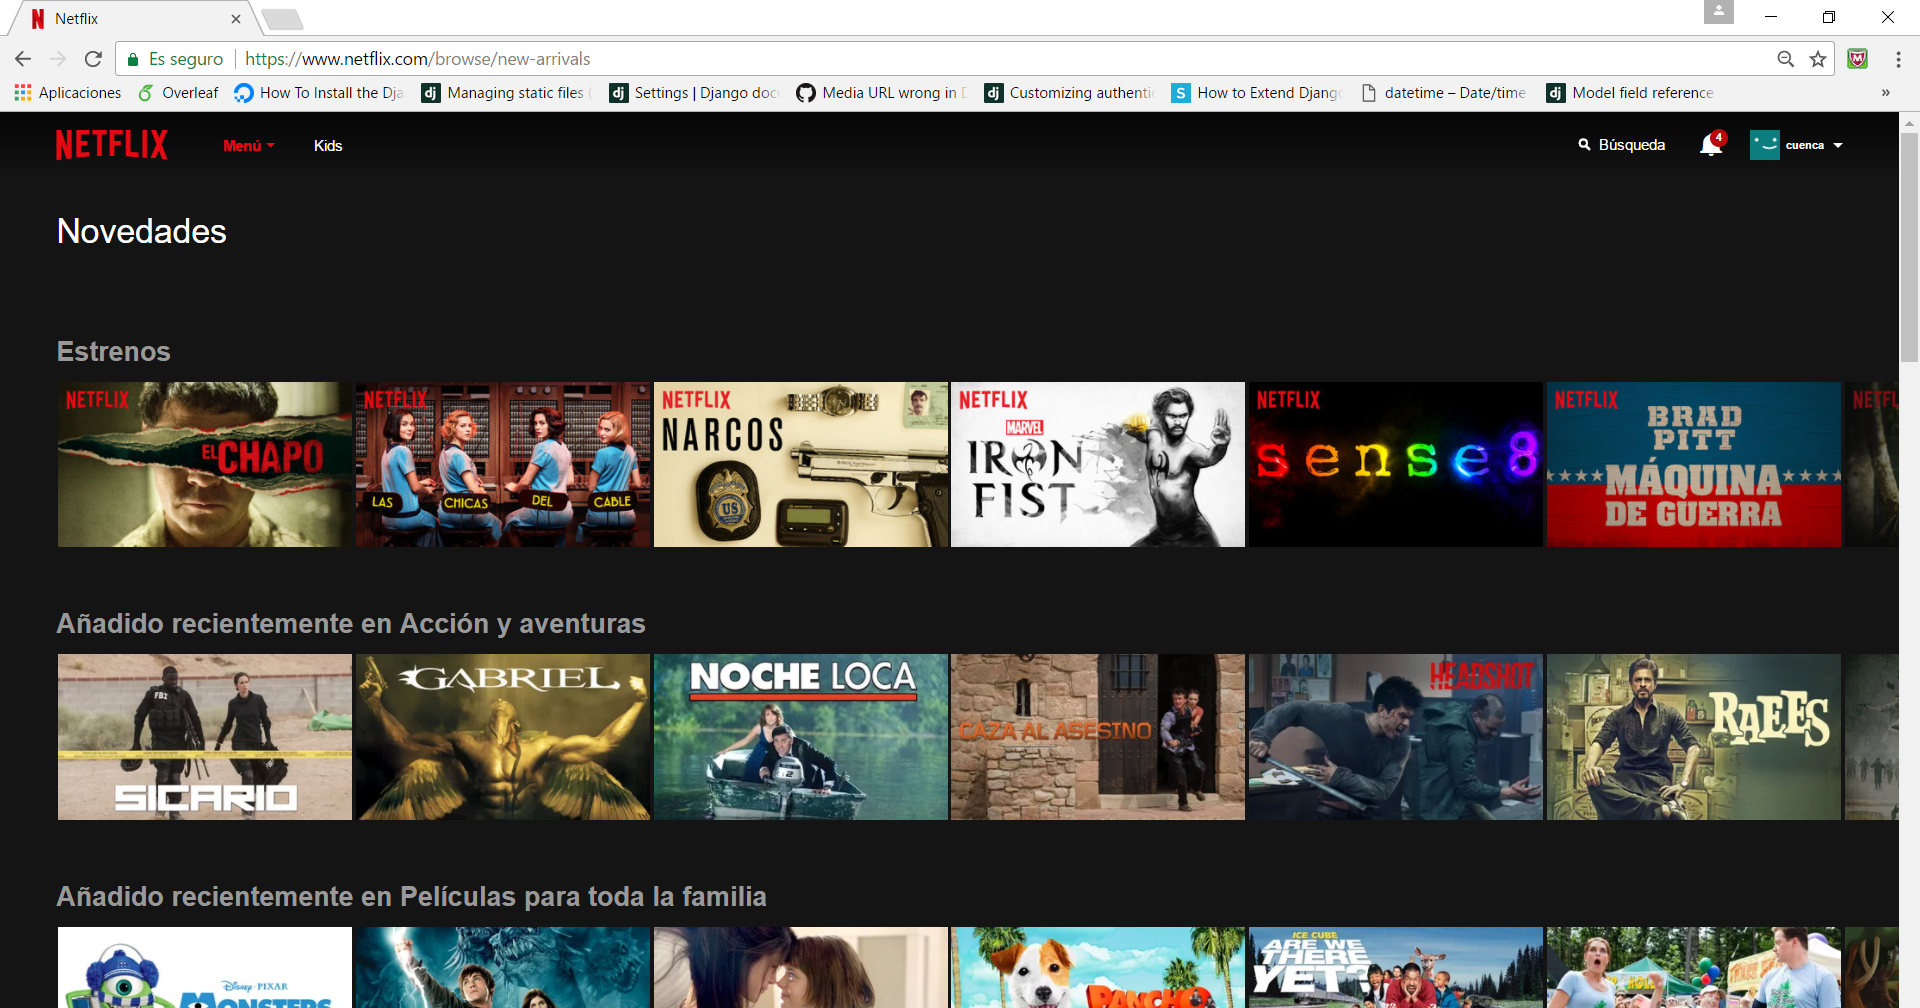
\includegraphics[width=0.8\textwidth]{img/netflix.png}
%\end{figure}
%\end{center}
%\end{minipage}
%\end{hslide}

%%--------------------------------------------------------------
%%------- Transparencias de Objetivos
%%--------------------------------------------------------------
\begin{hslide}
\slsect{Objetivos}
EL TFG se centra en un entorno docente, donde se quiere exponer a los alumnos de la asignatura de Laboratorios de Tecnologías Audiovisuales en la Web de cuarto curso del grado de Sistemas Audiovisuales y Multimedia  a un conjunto variado de tecnologías web proponiéndoles cuatro practicas atractivas, que se pueden elaborar como aplicaciones tradicionales, de escritorio, pero también se pueden elaborar empleando tecnologías web, navegadores y clientes, siendo de este modo multiplataforma. Este objetivo global será estructurado en cuatro subobjetivos, correspondientes a cada una las siguientes cuatro prácticas.
Sub-objetivos:
\begin{enumerate}
\item  Crear el juego del comecocos en la web basado en tecnologías del cliente. Para la visualización se utilizara Canvas mientras que para la funcionalidad se utilizara JavaScript permitiendo ejecutar eventos del teclado, además de incluir audio.
\item Crear una versión multijugador del juego del comecocos basado en tecnologías de comunicación bidireccional en tiempo real. Su diseño se basara en un servidor creado en NodeJS y WebSokects como mecanismo de comunicación bidireccional entre los navegadores y el servidor.
\item Crear un sitio Web de una tienda basada en tecnologías de servidor con manejo de base de datos. Su diseño se basara en el entorno Django para la gestión del sitio de Web y como BBDD MySQL.
\item Crear una aplicación de Videoconferencia Peer-to-Peer entre navegadores basada en tecnologías de comunicación audiovisual. Su diseño se realizara con WebRTC como tecnología core y NodeJS para la creación del servidor auxiliar.
\end{enumerate}
\end{hslide}


%%--------------------------------------------------------------
%%------- Transparencias Infraestructura
%%--------------------------------------------------------------

\begin{hslide}
\slsect{Infraestructura}
\slsubsect{HTML5}
\end{hslide}

\begin{hslide}
\slsect{Infraestructura}
\slsubsect{Lenguaje JavaScript}
weqeqweqweqweqweqweqewq
\end{hslide}

\begin{hslide}
\slsect{Infraestructura}
\slsubsect{Bibliotecas}
\begin{itemize}
\item \textbf{Jquery}
\item \textbf{Bootstrap}
\end{itemize}
\end{hslide}

\begin{hslide}
\slsect{Infraestructura}
\slsubsect{Entorno de servidor}
\begin{itemize}
\item \textbf{NodeJS}:
\item \textbf{Django}:
\end{itemize}
\end{hslide}

\begin{hslide}
\slsect{Infraestructura}
\slsubsect{Base de datos en aplicaciones Web}
\begin{itemize}
\item \textbf{MySQL}
\end{itemize}
\end{hslide}


\begin{hslide}
\slsect{Infraestructura}
\slsubsect{WebRTC}
\begin{itemize}
\item \textbf{Servidor de señalización}:
\item \textbf{GetUserMedia}:
\item \textbf{RTCPeerConnection}:
\item \textbf{RTCDataChannel}:

\end{itemize}
\end{hslide}


\begin{hslide}
\slsect{Infraestructura}
\slsubsect{Web Services}
\begin{itemize}
\item \textbf{WebServices Google Maps}:
\end{itemize}
\end{hslide}

%%--------------------------------------------------------------
%%------- Transparencias Comecocos Web
%%--------------------------------------------------------------

\begin{hslide}
\slsect{Comecocos Web}
\slsubsect{Enunciado}
La primera practica se centra en JavaScript haciendo énfasis en una aplicación web con mucho peso en el lado cliente. Se realiza la manipulación del DOM, gráficos 2D a través del elemento canvas e incorporar fuentes de audio a través del elemento audio.
\end{hslide}

\begin{hslide}
\slsect{Comecocos Web}
\slsubsect{Diseño de una solución}
\begin{minipage}{8cm}
\begin{center}
\begin{figure}
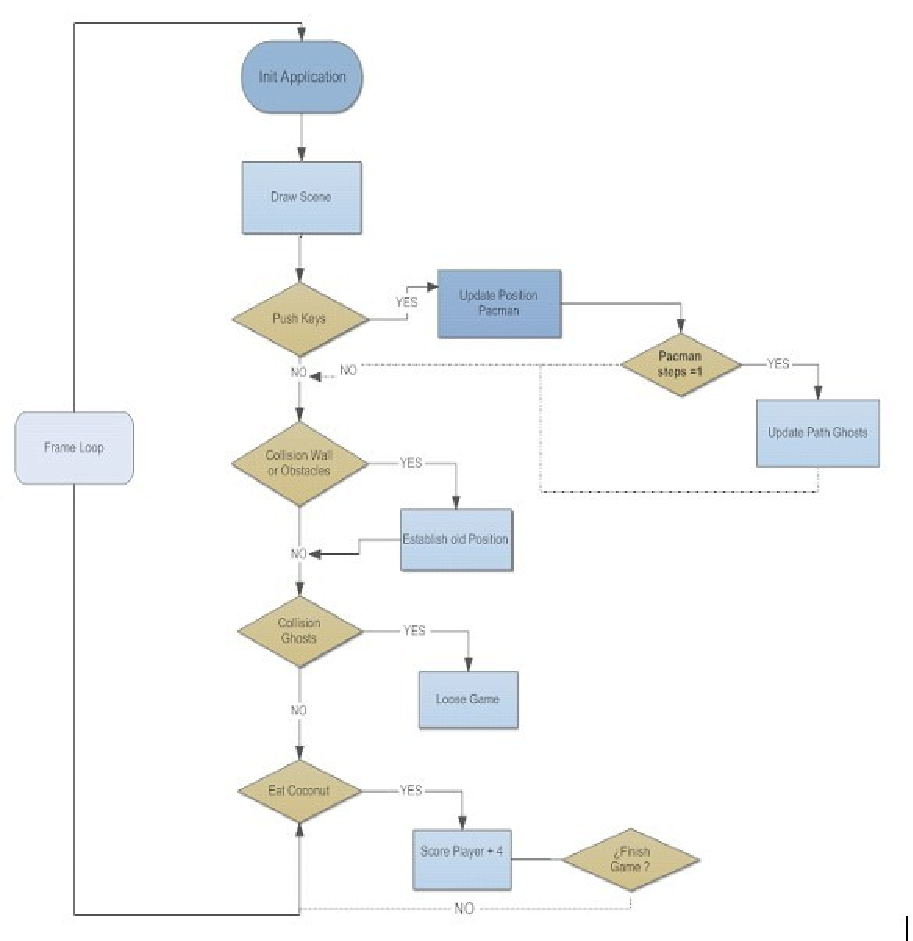
\includegraphics[width=7cm]{img/esquemaP1.pdf}
\end{figure}
\end{center}
\end{minipage}
\end{hslide}

\begin{hslide}
\slsect{Comecocos Web}
\slsubsect{Desarrollo area de  juego}
Este objeto es el encargado de generar y dibujar los elementos del juego. El objeto inicializa una serie de variables que hacen referencia a dichos elementos. 
\begin{itemize}
\item \textbf{Instancia de canvas}.
\item \textbf{Escenario y elementos}.
\item \textbf{Información de la partida}.
\item \textbf{Fin de Partida}.
\item \textbf{Movimiento}.
\end{itemize}
\begin{minipage}{8cm}
\begin{center}
\begin{figure}
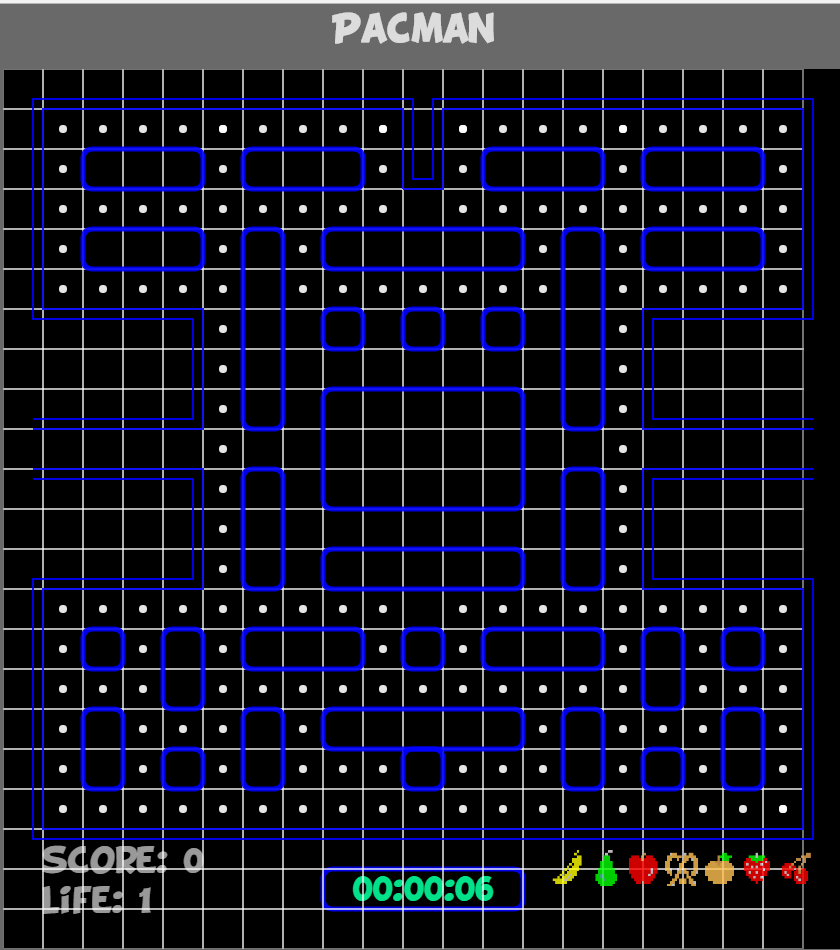
\includegraphics[width=6.5cm]{img/InfoGame.png}
\end{figure}
\end{center}
\end{minipage}
\end{hslide}

\begin{hslide}
\slsect{Comecocos Web}
\slsubsect{Desarrollo Pacman}
Es el protagonista del juego y el usuario interactúa moviéndolo por el escenario de juego. Al crear la instancia de objeto \texttt{Pacman(x, y, x\_map, y\_map)} se le pasa las coordenadas iniciales donde empieza la partida. Además, en su lógica es necesario comprobar diversos factores que afectan a su progreso en el juego que se incorporan dentro de la función \texttt{updateGameArea}. 
\begin{itemize}
\item \textbf{Detectar colisiones}.
\item \textbf{Comer Cocos}.
\item \textbf{Interacción movimiento}.
\item \textbf{Actualizar posición: canvas y mapa de juego}.
\item \textbf{Visualización}.
\end{itemize}
\end{hslide}

\begin{hslide}
\slsect{Comecocos Web}
\slsubsect{Desarrollo Fantasmas}
Definimos el objeto \texttt{Ghost} que contiene la lógica del comportamiento de los fantasmas que forman parte del juego. En el momento de instanciar el objeto \texttt{Ghost(x\_map, y\_map, name, speed, initMoment)} se pasan las coordenadas (x\_map,y\_map) posición, el nombre, su velocidad y el número de cocos que Pacman tiene que haber comido para salir a perseguirlo. Las distintas funciones del objeto se emplean dentro de la función \texttt{updateGameArea}. 
\begin{minipage}{8cm}
\begin{center}
\begin{figure}
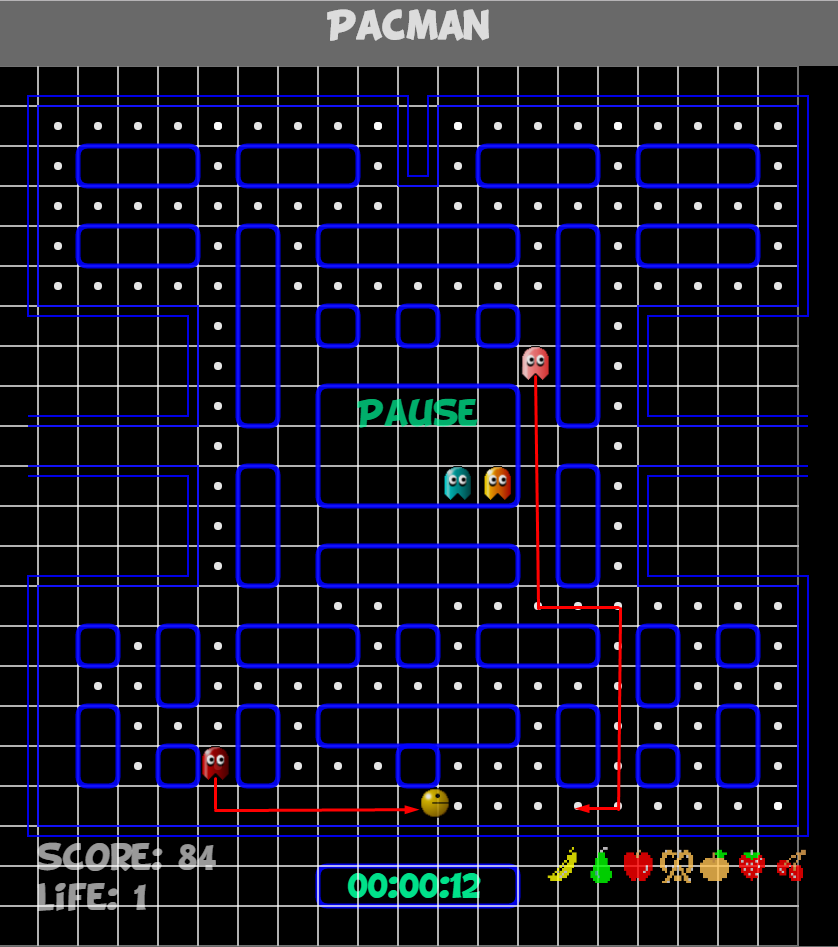
\includegraphics[width=6.5cm]{img/SeguimientoGhost.png}
\end{figure}
\end{center}
\end{minipage}
\begin{itemize}
\item \textbf{Persecución Pacman}.
\item \textbf{Actualizar objetivo}.
\item \textbf{Actualizar posición}.
\item \textbf{Visualización}.
\end{itemize}
\end{hslide}


\begin{hslide}
\slsect{Comecocos Web}
\slsubsect{Validacion experimental}
\begin{itemize}
\item \textbf{WebServices Google Maps}: Simula sensores, actuadores, robots,... en mundos virtuales.
\end{itemize}
\end{hslide}

%%--------------------------------------------------------------
%%------- Comecocos Web Multijugador
%%--------------------------------------------------------------

\begin{hslide}
\slsect{Comecocos Web multijugador}
\slsubsect{Enunciado}
Se pide desarrollar el juego del comecocos multijugador por medio de un interfaz web permitiendo establecer una partida con múltiples usuarios empleando Websockets. El escenario de juego y los cocos serán comunes para todos los jugadores quienes dispondrán de su propio comecocos que tiene que tener asociado un fantasma.
\end{hslide}

\begin{hslide}
\slsect{Comecocos Web Multijugador}
\slsubsect{Diseño de una solucion}

\begin{minipage}{8cm}
\begin{center}
\begin{figure}
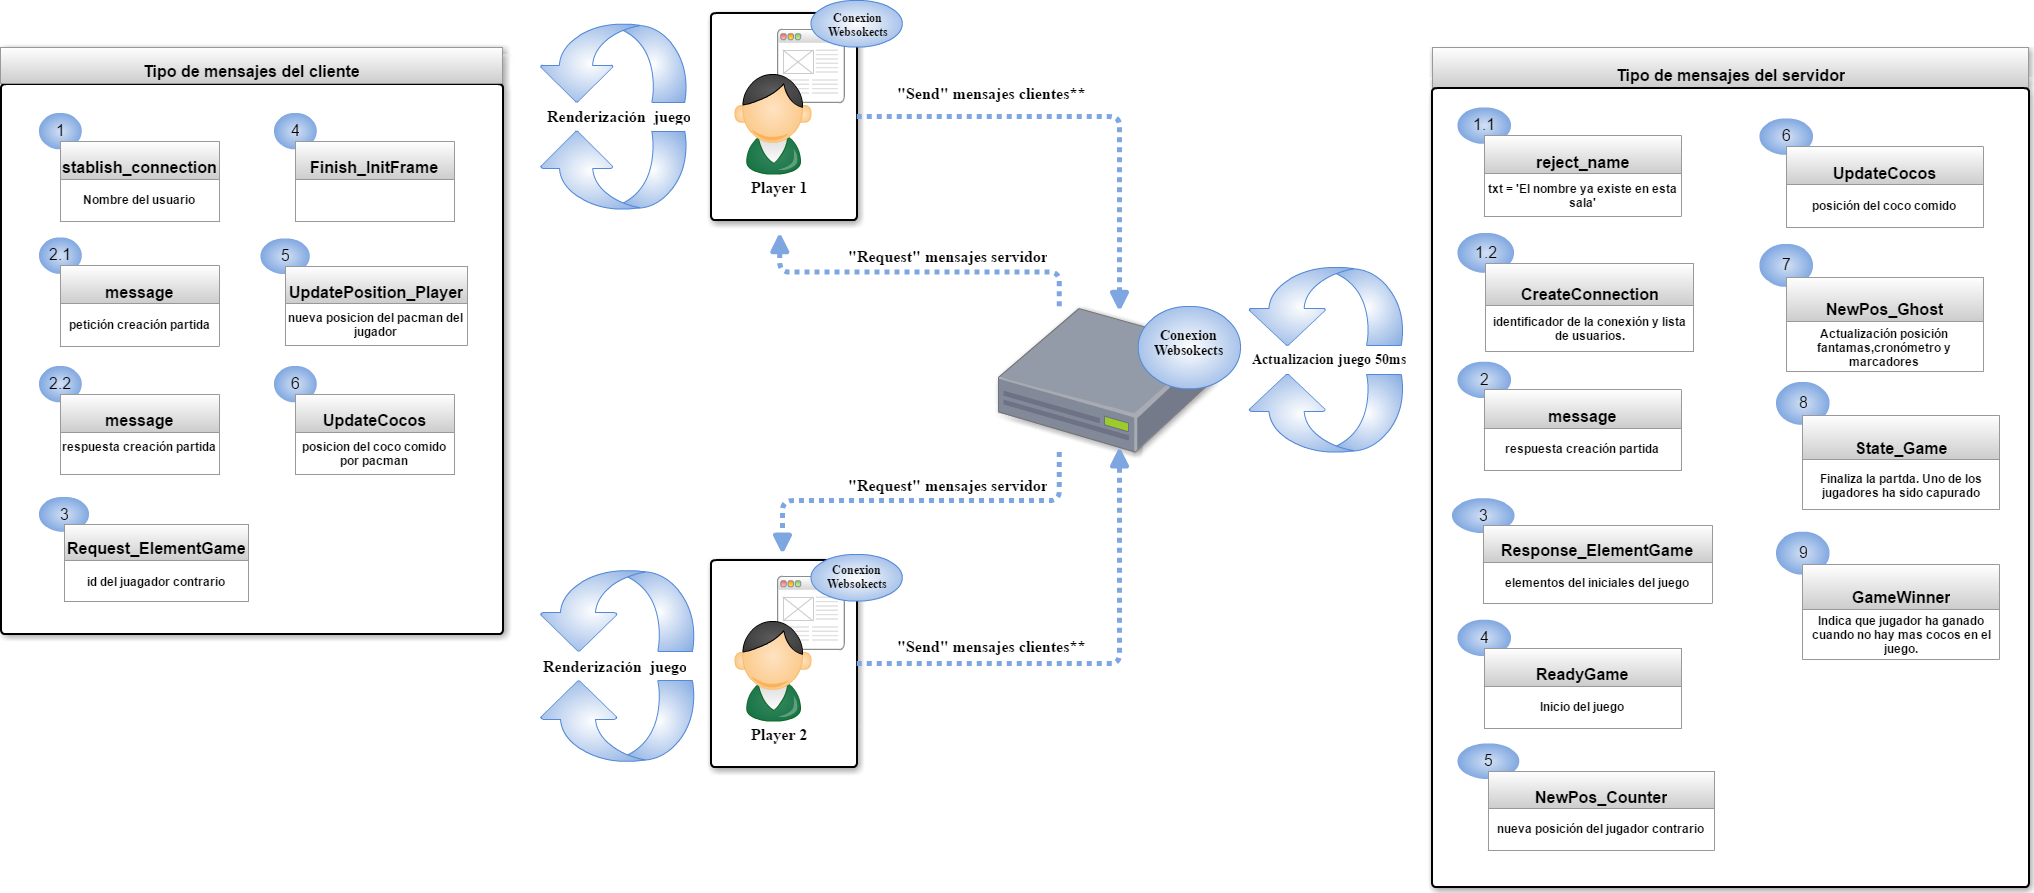
\includegraphics[width=12.2cm]{img/Esquema_Pacman_Multijugador.png}
\end{figure}
\end{center}
\end{minipage}
\end{hslide}

\begin{hslide}
\slsect{Comecocos Web Multijugador}
\slsubsect{Desarrollo servidor}
Proporciona el fichero html inicial que contiene la aplicación. Tras esto establece una comunicación WebSockets con los clientes. Al tener parte de la lógica del juego se genera un módulo que contenga los valores iniciales del juego como los cocos, obstáculo entre otros elementos y un objeto de tipo \texttt{Player} que contenga la posición del usuario y del fantasma correspondiente. Además,  por medio de la conexión WebSockets gestiona la entrada en la sala, inicio del juego y la actualización de los distintos elementos del juego.
\begin{itemize}
\item \textbf{WebServices Google Maps}: Simula sensores, actuadores, robots,... en mundos virtuales.
\end{itemize}
\end{hslide}

\begin{hslide}
\slsect{Comecocos Web Multijugador}
\slsubsect{Desarrollo cliente}
Establece conexión WebSockets con el servidor para intercambiar mensajes sobre el acceso a la sala de juego y los distintos estados del juego. Además, se encarga de dibujar el escenario del juego, fantasmas, jugadores e información de la partida con la información recibida del servidor. Además, gestiona el movimiento del personaje por medio de los eventos del teclado y los valida.

\end{hslide}

\begin{hslide}
\slsect{Comecocos Web Multijugador}
\slsubsect{Validacion experimental}

\end{hslide}


%%--------------------------------------------------------------
%%------- Comecocos Web Sitio Web de una tienda
%%--------------------------------------------------------------

\begin{hslide}
\slsect{Sitio Web de una tienda}
\slsubsect{Enunciado}
\end{hslide}



\begin{hslide}
\slsect{Sitio Web de una tienda}
\slsubsect{Desarrollo lado servidor}
Esta capa se encarga de buscar información en la BBDD de acuerdo a las peti-ciones que recibe y de entregar la información a los ficheros html correspondientespara que el navegador se encargue de visualizarlos
\begin{itemize}
\item \textbf{Conexión Django-BBDD}:
\item \textbf{Formularios}:
\item \textbf{Diseño de URL's y vistas}:
\end{itemize}
\end{hslide}

\begin{hslide}
\slsect{Sitio Web de una tienda}
\slsubsect{Desarrollo lado cliente}
Esta capa de la aplicación se encarga del diseño de los ficheros html donde sevuelca la información de las vistas. Para acceder a la información es necesario apli-car el lenguaje de plantillas de Django. La figura 6.8 muestra cada uno de los fiche-ros (html y/o js) creados para la aplicación.Ahora pasamos a explicar el contenido de cada uno de los ficheros tanto la apa-riencia como la funcionalidad.
\begin{itemize}
\item \textbf{Home}:
\item \textbf{Barra de navegación}:
\item \textbf{Cantantes}:
\item \textbf{Eventos}:
\item \textbf{Carrito de la compra}:
\item \textbf{Orden de compra}:
\end{itemize}
\begin{minipage}{8cm}
\begin{center}
\begin{figure}
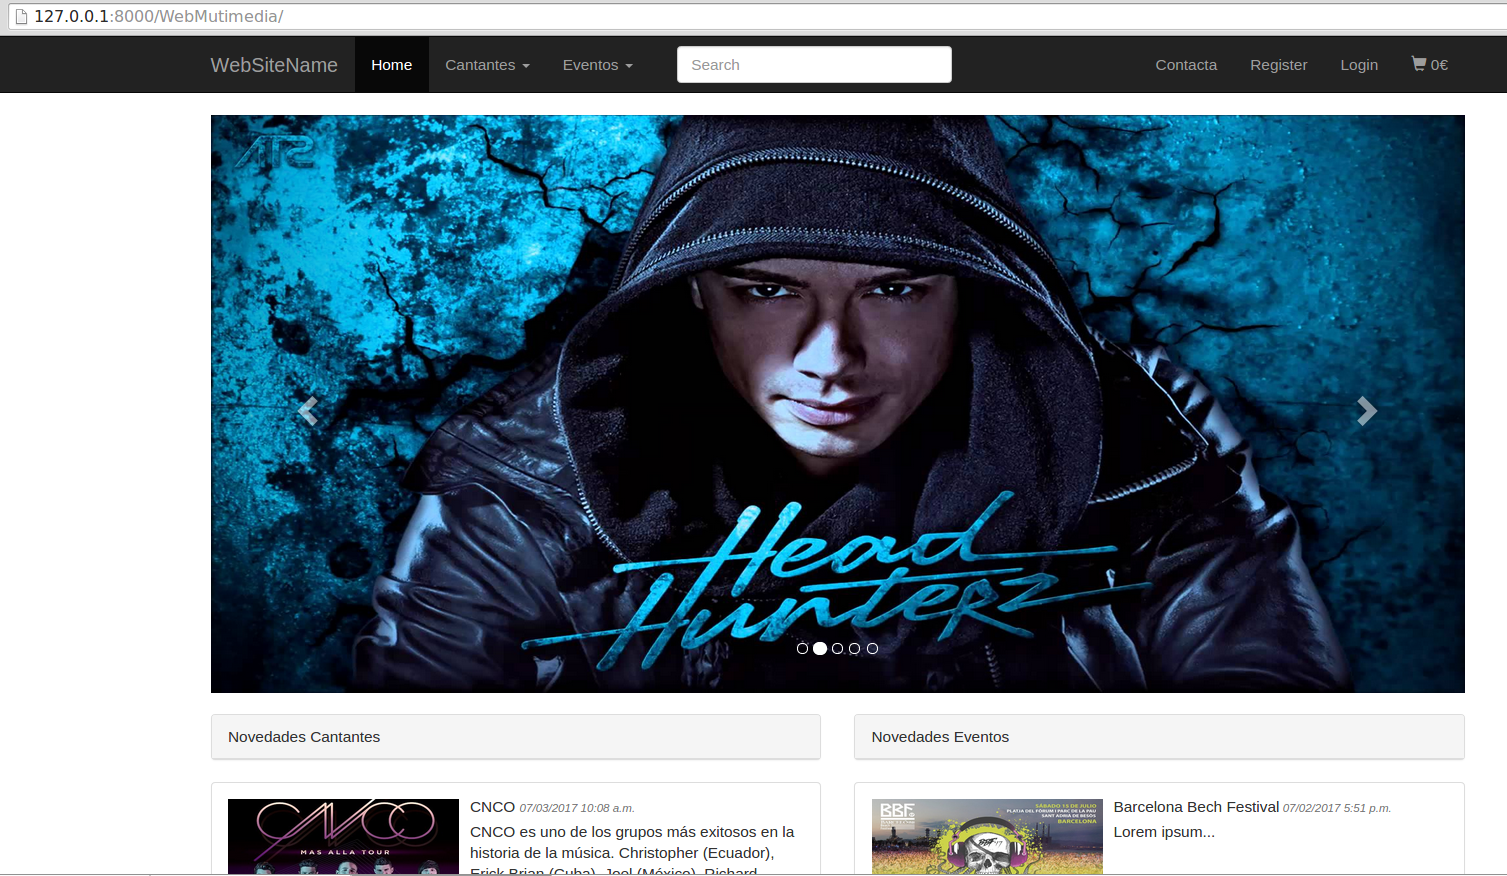
\includegraphics[width=11.5cm]{img/Page_1.png}
\end{figure}
\end{center}
\end{minipage}
\end{hslide}

\begin{hslide}
\slsect{Sitio Web de una tienda}
\slsubsect{Validacion experimental}
\end{hslide}

%%--------------------------------------------------------------
%%------- Comecocos Web Sitio Web de una tienda
%%--------------------------------------------------------------

\begin{hslide}
\slsect{Aplicación web de videoconferencia con WebRTC}
\slsubsect{Enunciado}
\end{hslide}

\begin{hslide}
\slsect{Aplicación web de videoconferencia con WebRTC}
\slsubsect{Diseño de una solución}
\begin{minipage}{8cm}
\begin{center}
\begin{figure}
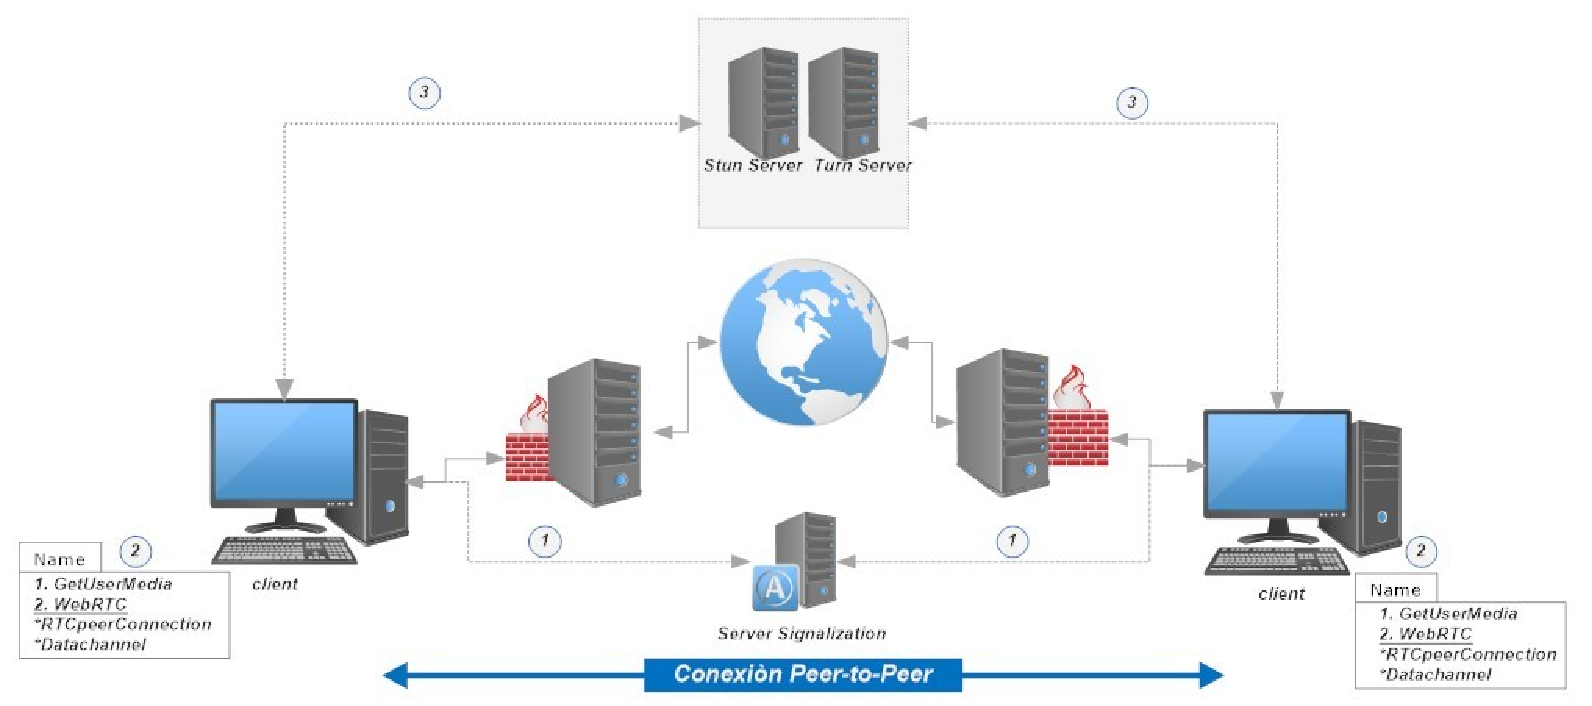
\includegraphics[width=12cm]{img/ComunnicacionWebRTC.pdf}
\end{figure}
\end{center}
\end{minipage}
\end{hslide}

\begin{hslide}
\slsect{Aplicación web de videoconferencia con WebRTC}
\slsubsect{Servidor de señalización}
\begin{itemize}
\item \textbf{Inicio de conexión}:
\item \textbf{Mensajes señalizacioón cliente}:
\end{itemize}
\end{hslide}

\begin{hslide}
\slsect{Aplicación web de videoconferencia con WebRTC}
\slsubsect{Desarrollo del cliente}
\begin{itemize}
\item \textbf{Inicio de conexión}:
\item \textbf{Conexion WebRTC para chat y envió de ficheros}:
\end{itemize}
\end{hslide}

\begin{hslide}
\slsect{Aplicación web de videoconferencia con WebRTC}
\slsubsect{Validacion experimental}
\end{hslide}


%%--------------------------------------------------------------
%%------- transpans Conclusiones
%%--------------------------------------------------------------

\begin{hslide}
\slsect{Conclusiones}
\begin{itemize}
\item \textbf{Concluciones}:
\item \textbf{Trabajos futuros}:
\end{itemize}
\end{hslide}

%%--------------------------------------------------------------
%%------- Transparencias Enlaces
%%--------------------------------------------------------------
\begin{hslide}
\slsect{Enlaces}
\begin{itemize}
\item Mediawiki: \url{http://jderobot.org/Walter-tfg}
\item Repositorio:\\ \url{https://github.com/RoboticsURJC-students/2015-TFG-Walter-Cuenca}
\end{itemize}
\end{hslide}

\end{document}